% Made up for the tikra benchmark.
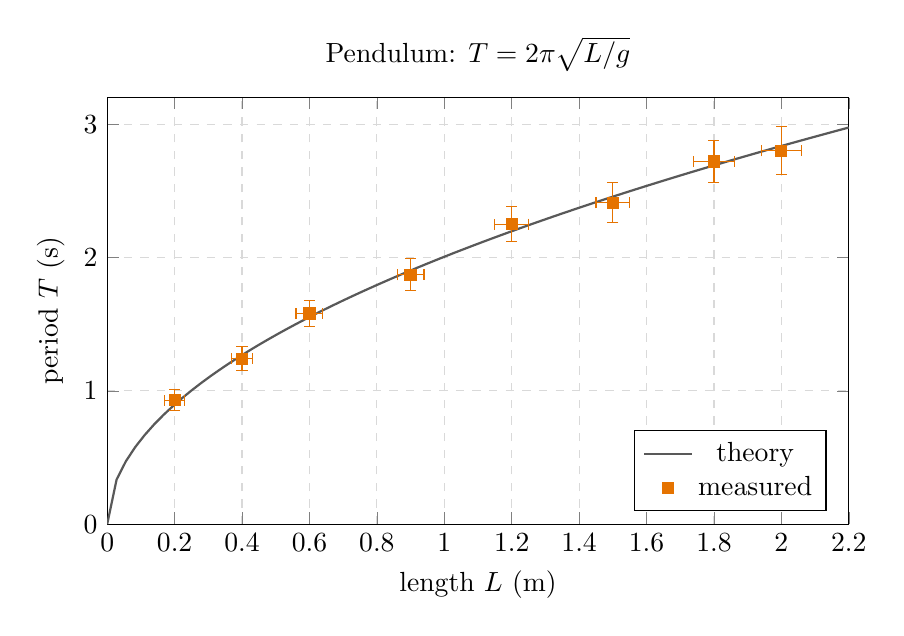
\begin{tikzpicture}
\begin{axis}[width=11cm, height=7cm, xmin=0, xmax=2.2, ymin=0, ymax=3.2,
    xlabel={length $L$ (m)}, ylabel={period $T$ (s)}, grid=major, grid style={dashed, gray!30},
    legend pos=south east, title={Pendulum: $T = 2\pi\sqrt{L/g}$}]
  \addplot[domain=0:2.2, samples=80, thick, gray!70!black] {2*pi*sqrt(x/9.81)};
  \addlegendentry{theory}
  \addplot[only marks, mark=square*, mark size=2pt, orange!90!black,
      error bars/.cd, y dir=both, y explicit, x dir=both, x explicit]
    coordinates {
      (0.2,0.93)  +- (0.03,0.08)
      (0.4,1.24)  +- (0.03,0.09)
      (0.6,1.58)  +- (0.04,0.10)
      (0.9,1.87)  +- (0.04,0.12)
      (1.2,2.25)  +- (0.05,0.13)
      (1.5,2.41)  +- (0.05,0.15)
      (1.8,2.72)  +- (0.06,0.16)
      (2.0,2.80)  +- (0.06,0.18)
    };
  \addlegendentry{measured}
\end{axis}
\end{tikzpicture}
